\section{Preliminary Data}

\begin{Figure}
    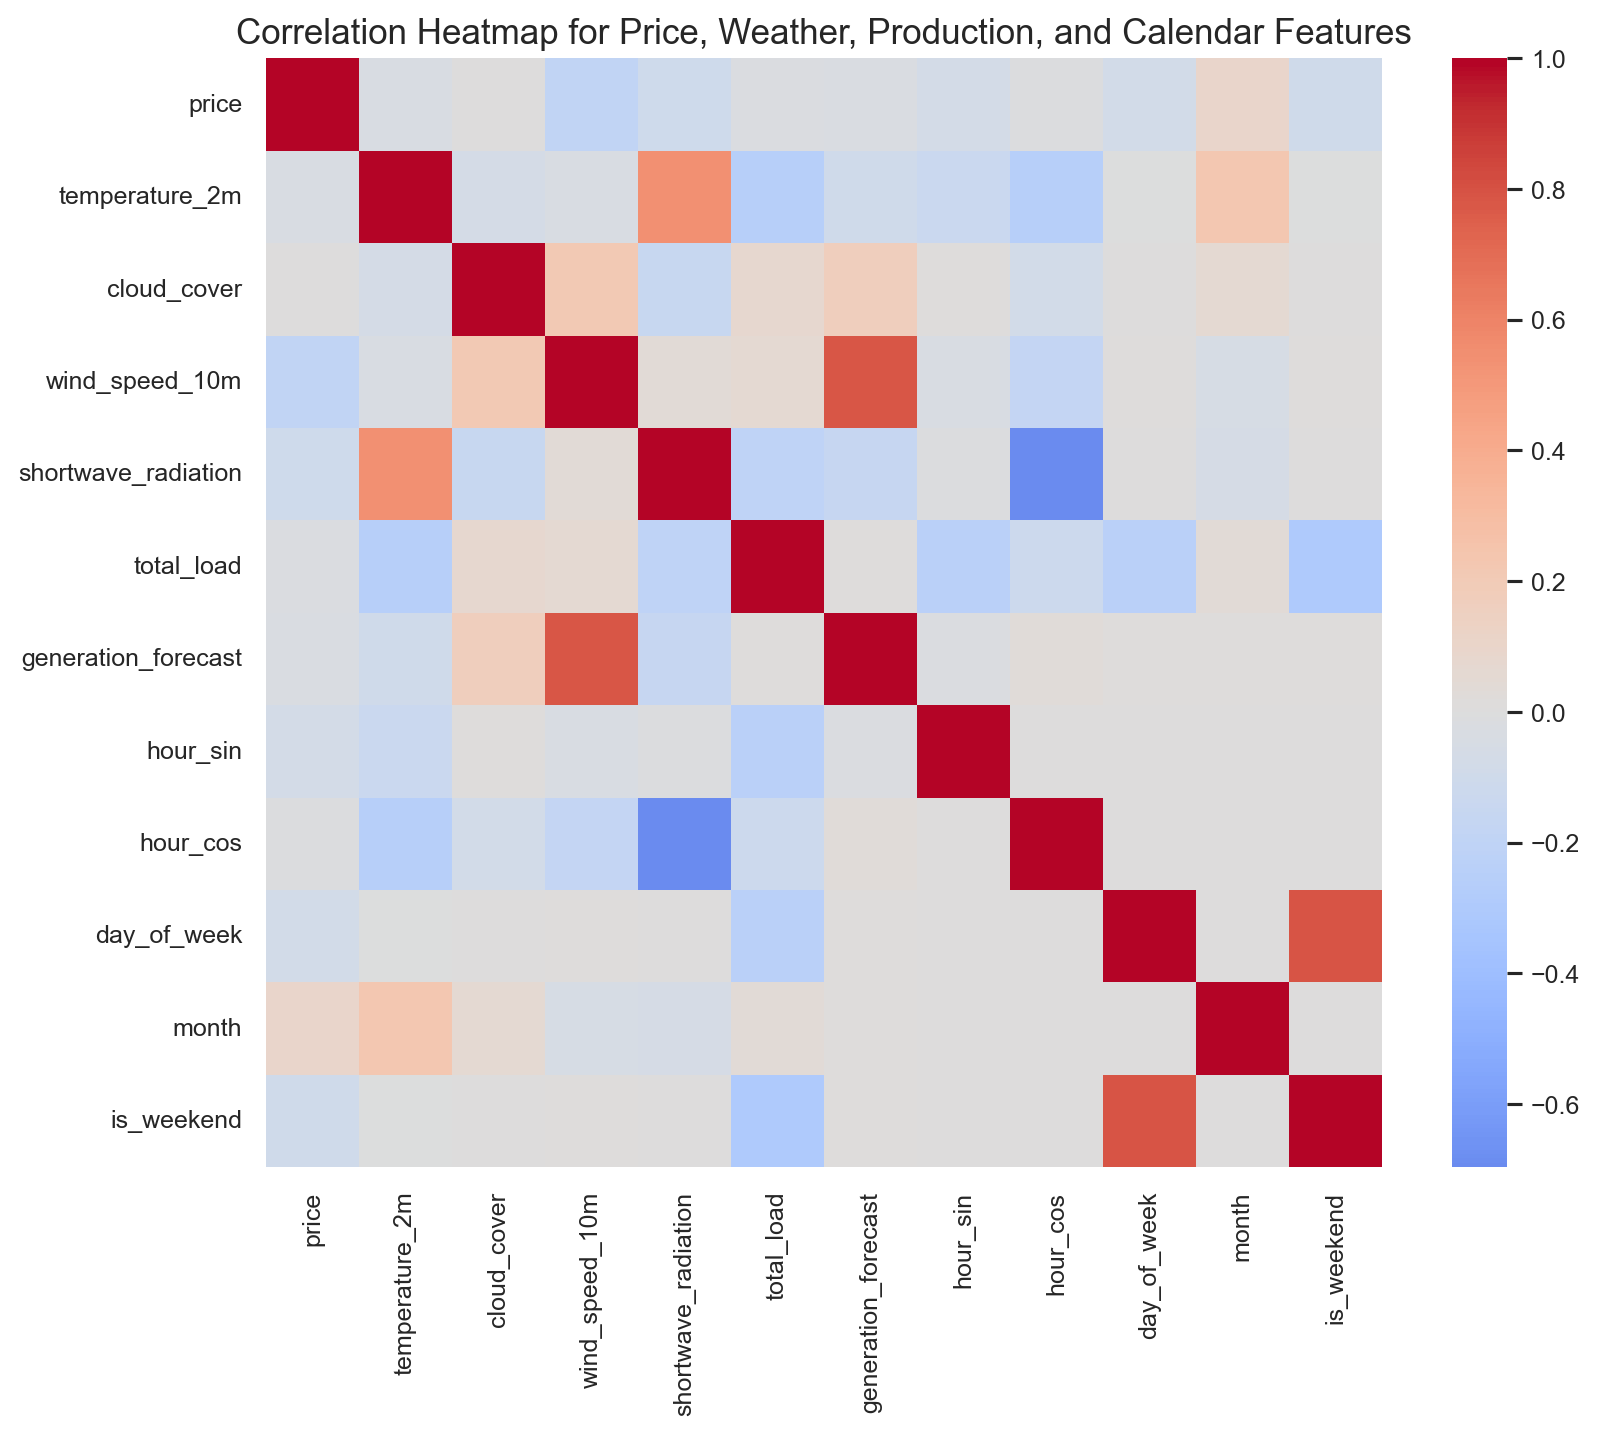
\includegraphics[width=\linewidth]{Figures/correlation_heatmap_weather_production_price.png}
    \captionof{figure}{Heatmap of correlation between features}\label{fig.corrHeat}
\end{Figure}

A preliminary analysis of the features in our dataset confirms some of the presumptions gathered from the literature; that price is inversely correlated to wind speed, with shortwave radiation also being slightly inversely correlated, as seen on Fig.\ref{fig.corrHeat}.
Its rather curious to observe the week correlation between load and price.

\begin{Figure}
    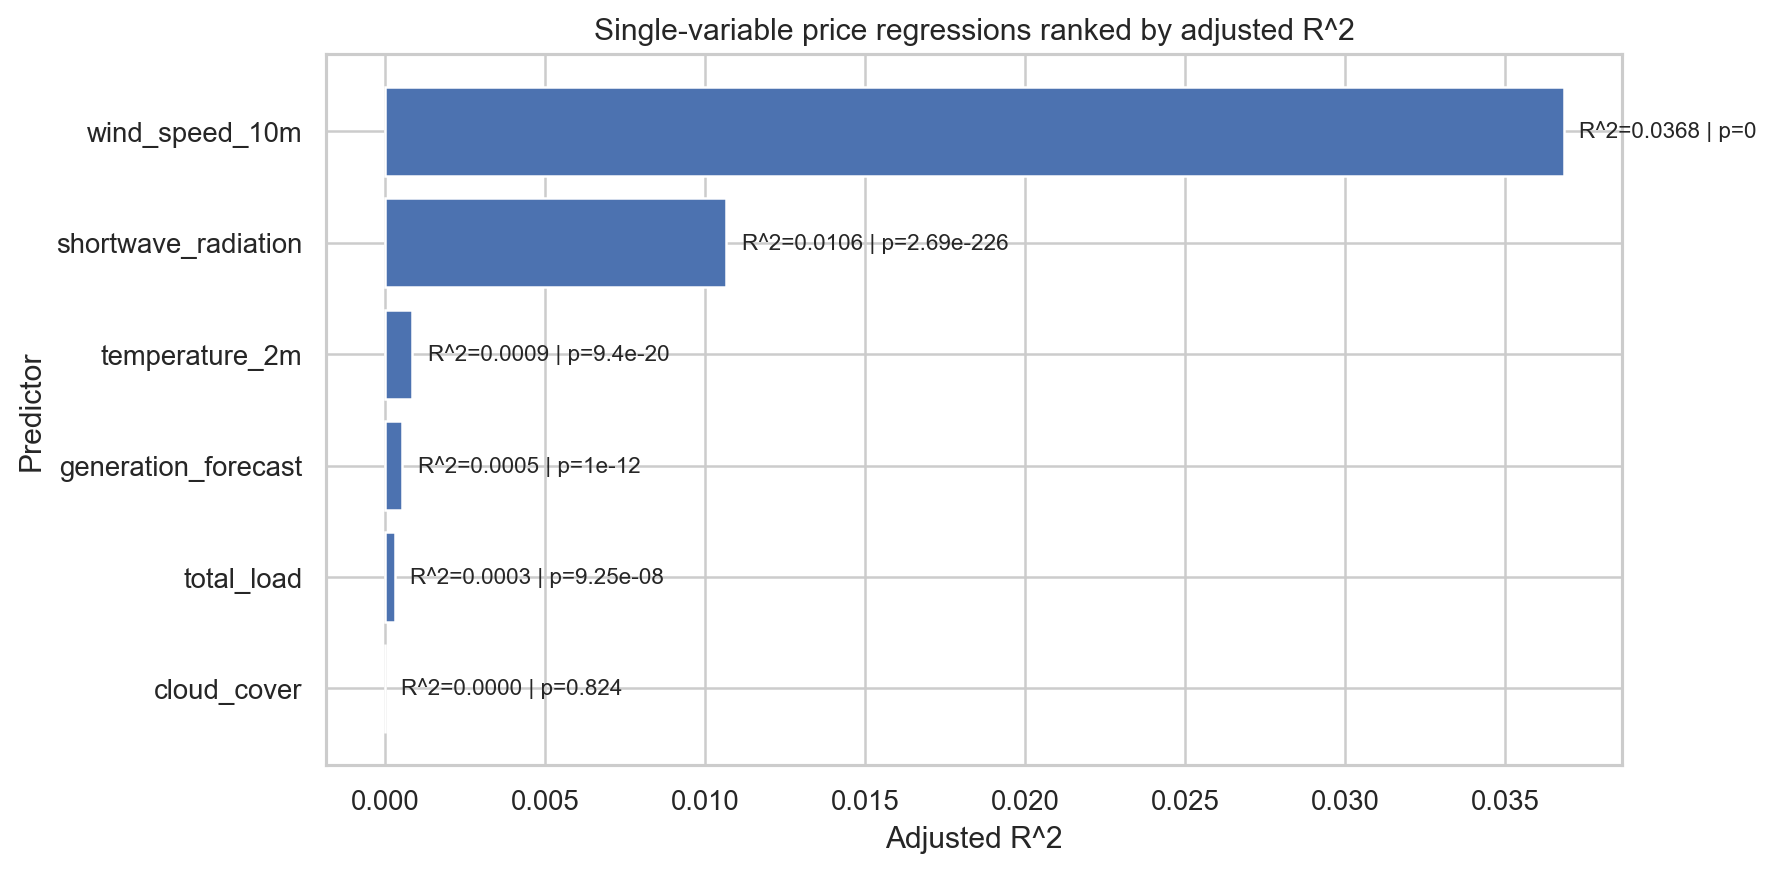
\includegraphics[width=\linewidth]{Figures/notebook_price_single_variable_regression_ranking.png}
    \captionof{figure}{Statistical significance per feature}\label{fig.pValue}
\end{Figure}
    
Similarly, wind speed, solar radiance, temperature, energy generation and load all appear to be statistically significant towards price (Fig.\ref{fig.pValue}).

\begin{Figure}
    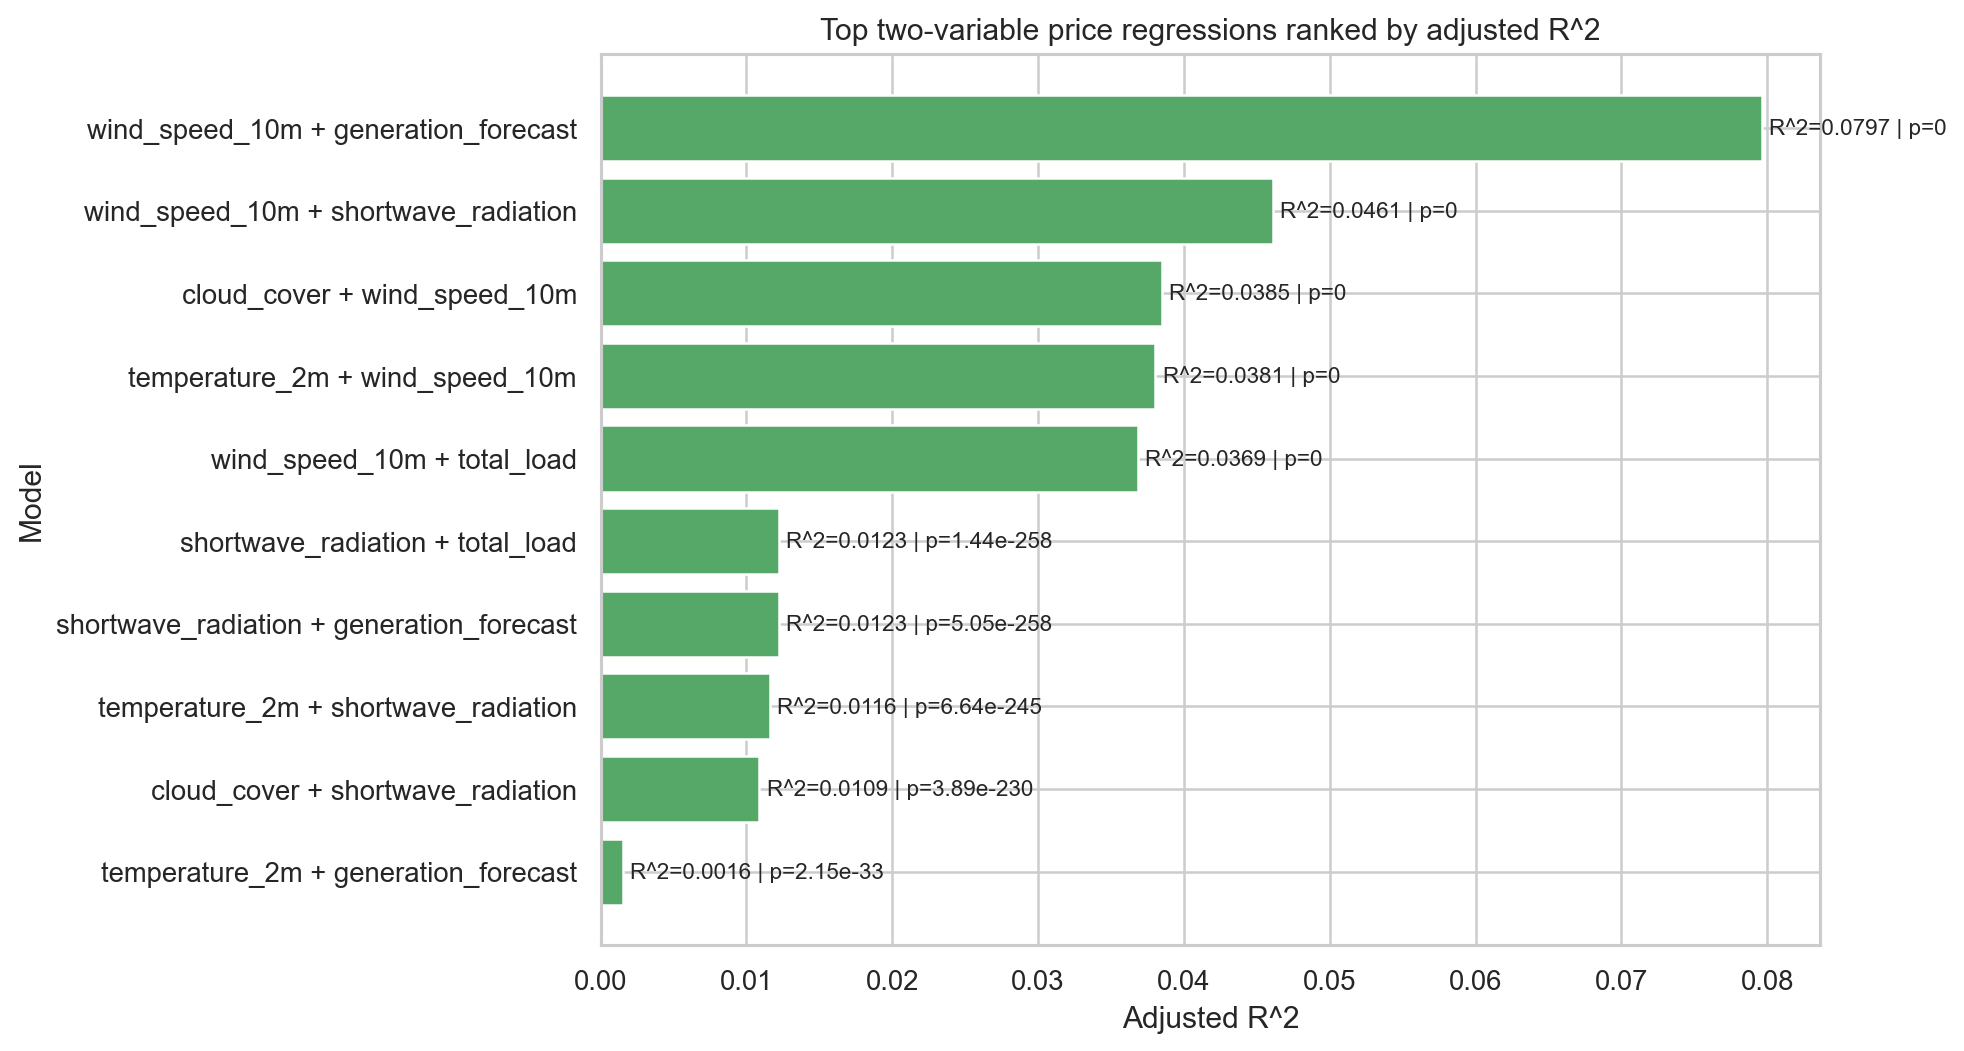
\includegraphics[width=\linewidth]{Figures/notebook_price_two_variable_regression_ranking.png}
    \captionof{figure}{Statistical significance per feature pair}\label{fig.compountpValue}
\end{Figure}

But interestingly, the combination of wind speed and overall generation seem to be more statistically significant, and hold greater explanatory power, than a combination of wind and solar.
This interpretation is supported by Fig.\ref{fig.corrHeat}, which shows that wind speed and generation forecast are closely correlated, meaning that wind power makes up a sizable chunk of the energy produced, when
the conditions allow for it. Besides, combinations of different weather features are all statistically significant.